\documentclass{article}
\usepackage[a4paper]{geometry}
\usepackage[utf8]{inputenc}
\DeclareUnicodeCharacter{00A0}{ }
\usepackage[english, italian]{babel}
\usepackage{parskip}
\usepackage{etaremune}
\usepackage{appendix}
\renewcommand\appendixtocname{Appendici}
\setcounter{secnumdepth}{4}
\setcounter{tocdepth}{4}
\usepackage[usenames,dvipsnames]{color}
\usepackage{titlesec}
\usepackage{float}
\usepackage[colorlinks=true]{hyperref}
\hypersetup{
    colorlinks=true,
    citecolor=black,
    filecolor=black,
    linkcolor=black,
    urlcolor=blue
}
\usepackage{breakurl}
\usepackage{graphicx}
\usepackage{lastpage}
\usepackage{longtable}
\usepackage{booktabs}
\usepackage{tabularx}
\usepackage{multirow}
\usepackage{longtable}
\usepackage[table]{xcolor}
\usepackage{tabu}
\setlength{\tabulinesep}{6pt}
\usepackage{array}
\usepackage{ragged2e}
\newcolumntype{P}[1]{>{\RaggedRight\hspace{0pt}}p{#1}}
\usepackage{fancyhdr}
\usepackage{textcomp}
\usepackage{changepage}
\usepackage{pgfplots}
\usepackage{tikz}
\usepackage{grffile}
\usepackage{rotating}
\usepackage{calc}
\fancypagestyle{plain}{
	% cancella tutti i campi di intestazione e piè di pagina
	\fancyhf{}

	\lhead{
		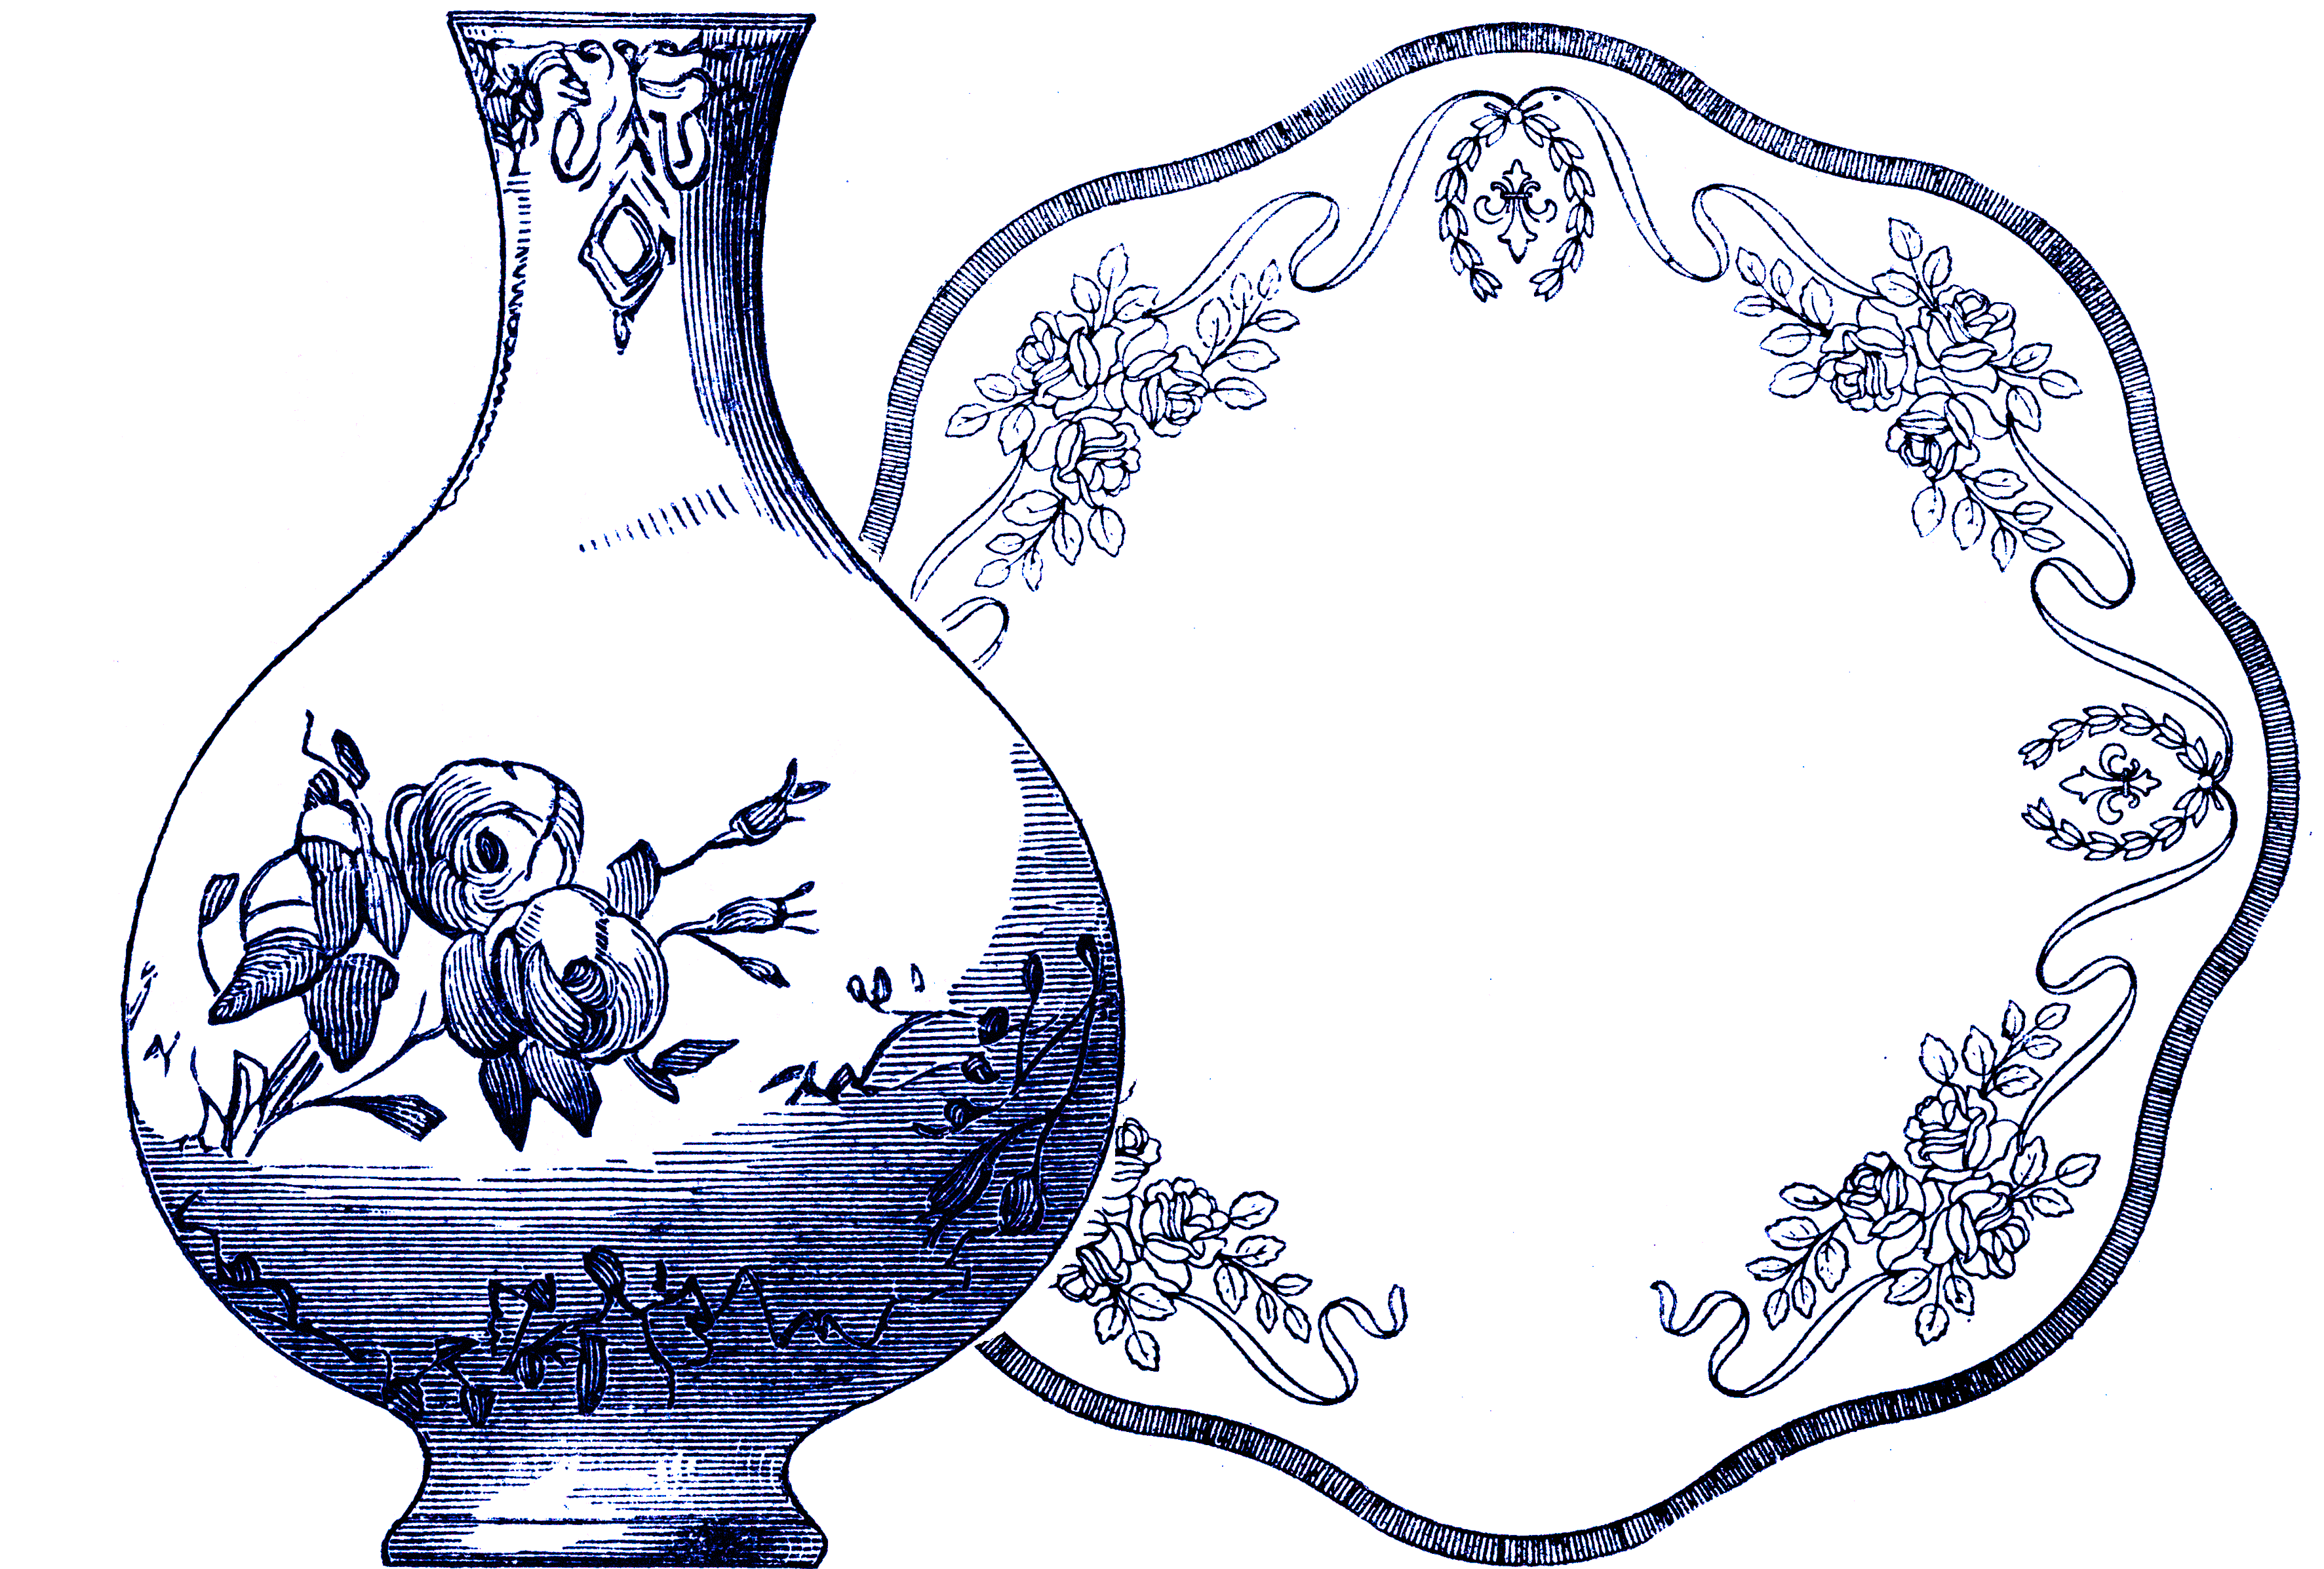
\includegraphics[height=1.5cm, width=1.5cm, keepaspectratio=true]{logo.png}
		\parbox[b]{10cm}{
			\emph{\ProjectName{}} \vspace{7pt}
		}
	}
	\chead{}
	\rhead{
		\slshape \leftmark
	}

	\lfoot{
		\ProjectName{}
	}
	\rfoot{Pagina \thepage{} di \pageref{LastPage}}
	\renewcommand{\headrulewidth}{0.3pt}
	\renewcommand{\footrulewidth}{0.3pt}
}
\setlength{\headheight}{30pt}
\pagestyle{plain}
\usepackage{listings}
\lstset{
  extendedchars=true,          % lets you use non-ASCII characters
  inputencoding=utf8,   % converte i caratteri utf8 in latin1, richiede \usepackage{listingsutf8} anzichè listings
  basicstyle=\ttfamily,        % the size of the fonts that are used for the code
  breakatwhitespace=false,     % sets if automatic breaks should only happen at whitespace
  breaklines=true,             % sets automatic line breaking
  captionpos=t,                % sets the caption-position to top
  commentstyle=\color{mygreen},   % comment style
  frame=none,               % adds a frame around the code
  keepspaces=true,            % keeps spaces in text, useful for keeping indentation of code (possibly needs columns=flexible)
  keywordstyle=\bfseries,     % keyword style
  numbers=none,               % where to put the line-numbers; possible values are (none, left, right)
  numbersep=5pt,              % how far the line-numbers are from the code
  numberstyle=\color{mygray}, % the style that is used for the line-numbers
  rulecolor=\color{black},    % if not set, the frame-color may be changed on line-breaks within not-black text (e.g. comments (green here))
  showspaces=false,           % show spaces everywhere adding particular underscores; it overrides 'showstringspaces'
  showstringspaces=false,     % underline spaces within strings only
  showtabs=false,             % show tabs within strings adding particular underscores
  stepnumber=5,               % the step between two line-numbers. If it's 1, each line will be numbered
  stringstyle=\color{red},    % string literal style
  tabsize=4,                  % sets default tabsize
  firstnumber=1      % visualizza i numeri dalla prima linea
}
\usepackage[T1]{fontenc}
\usepackage{lmodern}
\newcommand{\ProjectName}{LineaCasaBari}

\newcommand{\makeFrontPage}{
  % Declare new goemetry for the title page only.
  \newgeometry{top=3.5cm}
  
  \begin{titlepage}
  \begin{center}

  \begin{center}
  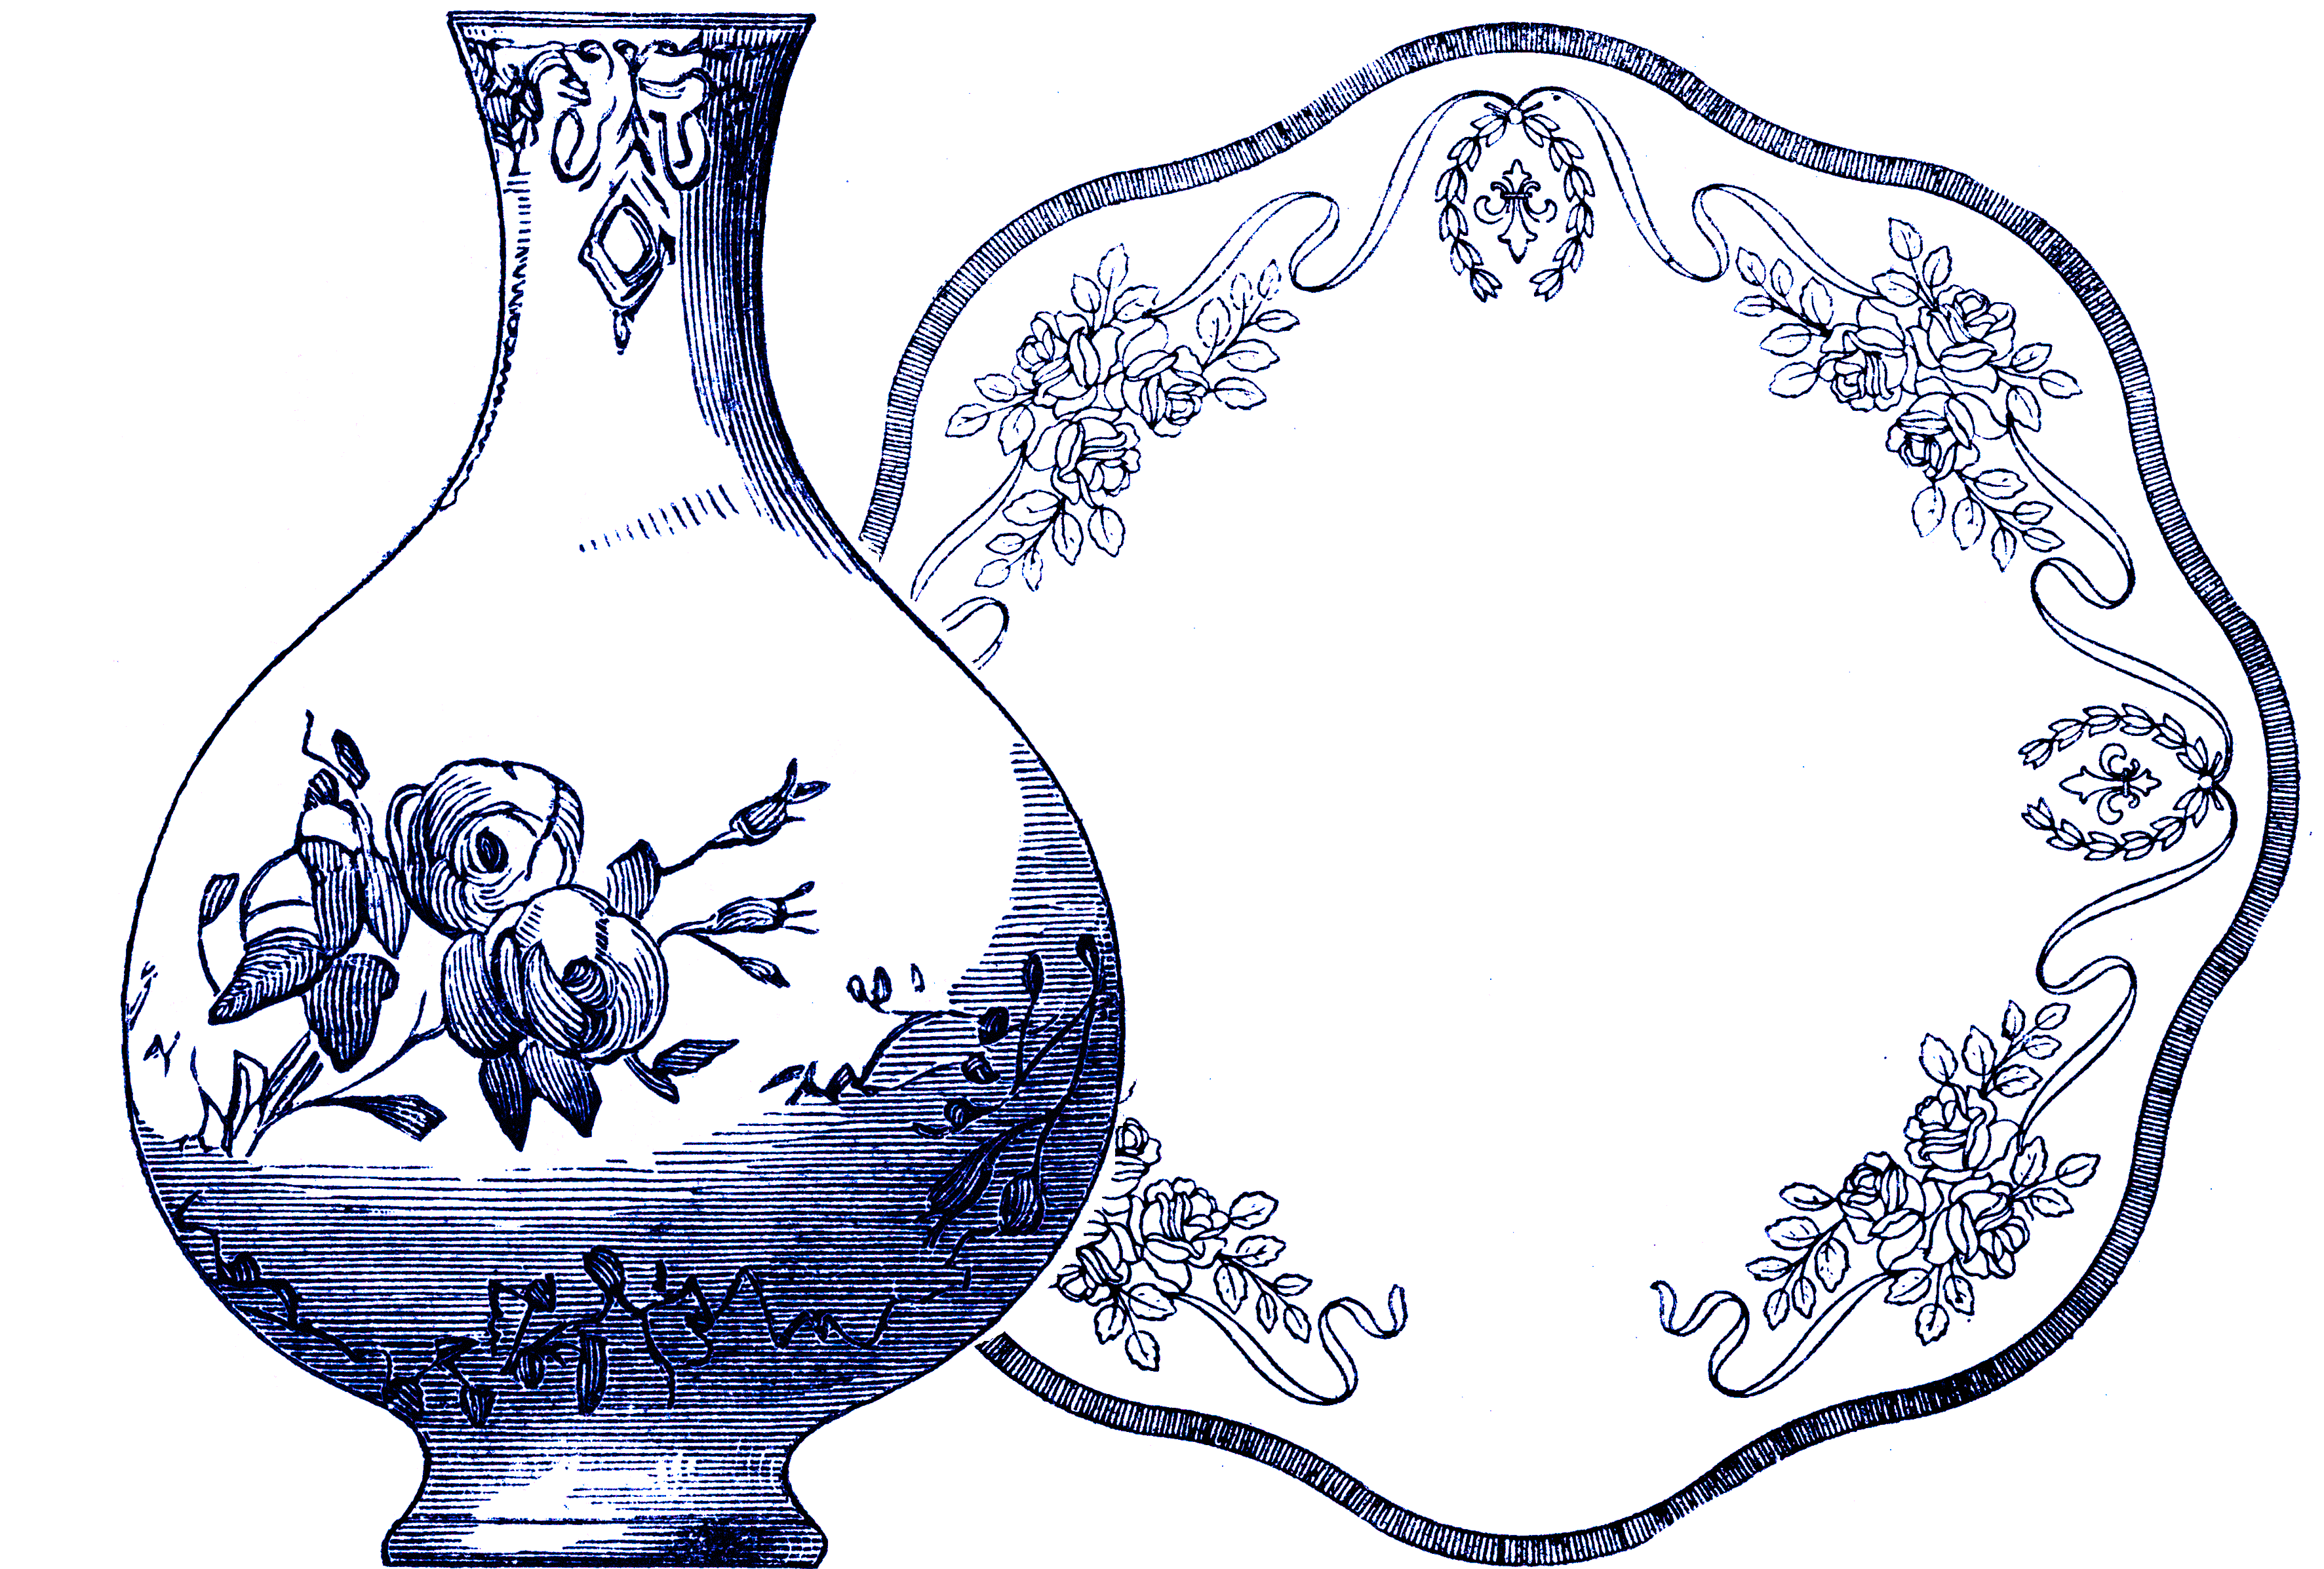
\includegraphics[width=10cm]{logo.png}
  \end{center}
  
  \vspace{1cm}

  \begin{Huge}
  \textbf{\ProjectName{}}
  \end{Huge}
  
  \vspace{11pt}

  \bgroup
  \def\arraystretch{1.3}
  \begin{tabular}{ r|l }
    \multicolumn{2}{c}{\textbf{Membri del gruppo}} \\
    \hline

    \textbf{Navid Taha} & 1069126 \\
    \textbf{Alice Sasso} & 1074588 \\
    \textbf{Lorenzo Ferrarin} & 1069405 \\
    \textbf{Alessandro Bari} & 1074356 \\
  \end{tabular}
  \egroup

  \vspace{22pt}

  \textbf{Informazioni sul sito} \\
  
  	\url{http://tecnologie-web.studenti.math.unipd.it/tecweb/~asasso/}
  	
  \vspace{5pt}
  \textbf{Referente} \\
  Navid Taha: navid.taha@studenti.unipd.it
  
  \vspace{7pt}  
  
  \textbf{Dati di accesso} \\
  
  
  
  login amministratore e utente
    
  
  \end{center}
  \end{titlepage}
  
  % Ends the declared geometry for the titlepage
  \restoregeometry
}

\begin{document}

\makeFrontPage
\clearpage
\tableofcontents
\clearpage

\section{Riferimenti informativi}
	\subparagraph{Link skipper}~
	
	Per la creazione del link skipper, con relativo supporto Javascript, si è seguita la seguente guida:
	\begin{center}
		\url{https://www.bignerdranch.com/blog/web-accessibility-skip-navigation-links/}
	\end{center}
	
	\subparagraph{Drawer}~
	
	Per la creazione del drawer o ``menu ad hamburger'' si è seguita la seguente guida:
	\begin{center}
		\url{http://www.designcouch.com/home/why/2014/04/23/pure-css-drawer-menu/}
	\end{center}

\section{Introduzione}
Il progetto ha lo scopo di sviluppare il sito web commerciale del negozio LineaCasaBari, operante nel settore della vendita di oggetti per la casa. \\
Il sito sarà composto da due principali aree: utente ed amministratore. \\
L'area amministratore consentirà la gestione del sito, tramite diverse funzionalità quali la rimozione di un utente, la rimozione/aggiunta/modifica di un prodotto, la modifica di un ordine e la rimozione/aggiunta/modifica di un annuncio. \\
L'area utente consentirà la consultazione di un elenco di prodotti acquistabili, la gestione del proprio account (modifica dei dati e degli indirizzi associati) e la visualizzazione di informazioni nel sito, tramite annunci e sezioni predisposte. \\
Lo sviluppo del sito è stato conferme alle predisposizioni degli standard W3C, ed inoltre si è mantenuta la separazione tra comportamento, struttura e presentazione.

\section{Analisi dei requisiti} % individuazione degli utenti e delle loro esigenze
	\subsection{Utenti esterni}
		\subsubsection{Utente non registrato}
		L'utente non registrato deve poter consultare il catalogo dei prodotti, tuttavia per l'acquisto dei prodotti dovrà registrarsi. Inoltre, ha la possibilità di consultare diverse informazioni, sia sui servizi proposti, che in generale sul sito e sulle novità di esso.  \\
		Le informazioni che cerca devono essere accessibili nel minor numero di click, in quanto è stato riscontrato che la permanenza di utente nel sito dipende da quanto tempo è necessario per reperire le informazioni utili.
		
		\subsubsection{Utente registrato}
		L'utente registrato visualizza la stessa versione del sito dell'utente non registrato, in modo da favorirne l'orientamento in esso. Tuttavia, ha la possibilità di effettuare degli ordini ed acquistare i prodotto offerti dal negozio. Inoltre, ha accesso alla sezione di gestione del proprio account, in cui ha la possibilità di modificare i dati del proprio account, aggiungere/modificare/rimuovere gli indirizzi di spedizione e consultare gli ordini effettuati; è presente anche la lista dei desideri, in cui l'utente può salvare i suoi articoli preferiti in modo da ritrovarli successivamente.

	\subsection{Utenti interni}
		\subsubsection{Amministratore}
		L'amministratore è la figura che gestisce il sito e lo mantiene. Si presume che non abbia intenzioni malevoli e che sia una persona esperta in tale ambito. Nonostante, sono stati previsti dei controlli, in modo da evitare eventuali distrazioni ed errori. \\
		L'amministratore ha la possibilità di gestire il sito effettuando l'accesso con delle credenziali speciali, immesse direttamente nel database dell'applicativo, nello stesso form di login utilizzato dagli utenti. Potrà successivamente accedere alla sezione di gestione del sito tramite un link posto nell'intestazione del sito. In tale sezione, è possibile gestire (modifica/ rimozione/ aggiunta) i dati del database interno del sito, che sono rappresentati dagli utenti, ordini, prodotti e annunci. \\
		Vengono mantenute le funzionalità offerte agli utenti, in modo da poterne verificare il funzionamento e la correttezza dal punto di vista dell'utente stesso, senza il bisogno di creare un altro account.

\section{Dati e informazioni} % progettazione della base informativa
	\subsection{Contenuti}
	Il sito ha la necessità di salvare e reperire, da un'apposita base di dati XML, i seguenti dati:
	\begin{itemize}
		\item \textbf{Annunci}: rappresentano i messaggi contenenti novità ed informazioni riguardanti il negozio. La gestione di questi dati viene riservata all'amministratore;
		\item \textbf{Utenti}: rappresentano gli utenti iscritti al sistema, compresi gli amministratori. Gli amministratore vengono individuati da un campo booleano e devono essere aggiunti a mano, modificando il file XML. La gestione di questi dati viene riservata all'amministratore;
		\item \textbf{Prodotti}: rappresentano i prodotti offerti dal negozio ed acquistabili dagli utenti registrati. La gestione di questi dati viene riservata all'amministratore;
		\item \textbf{Indirizzi}: rappresentano gli indirizzi di spedizione degli utenti. La gestione di questi dati viene riservata all'utente registrato;
		\item \textbf{Desideri}: rappresentano i prodotti aggiunti alla lista dei desideri da parte degli utenti. La gestione di questi dati viene riservata all'utente registrato;
		\item \textbf{Newsletter}: rappresentano le email degli utenti iscritti al servizio di invio di email informative riguardanti il negozio. La gestione di questi dati viene riservata all'utente registrato;
		\item \textbf{Ordini}: rappresentano il riepilogo degli acquisti effettuati dagli utenti con tutte le relative informazioni. La gestione di questi dati viene riservata sia agli utenti registrati, che all'amministratore;
		\item \textbf{Carrelli}: rappresentano gli ordini effettuati da parte degli utenti, ma ancora non acquistati. La gestione di questi dati viene riservata all'utente registrato.
	\end{itemize}
	
	\subsection{Schema dei dati}
	Lo schema XSD utilizzato per modellare i dati è \textbf{``Tende alla veneziana''}, il quale favorisce il riuso e la flessibilità. E' caratterizzato dal possedere un unico elemento globale, l'elemento radice, e tanti tipi nominali ciascuno dei quali contiene definizioni di elementi locali associati a tipi nominali ed esterni.
	
\section{Applicazioni e servizi} % progettazione delle funzionalità
	\subsection{Sezione amministratore}
	Sono state previste le seguenti funzionalità, volte alla gestione del sito, messe a disposizione dell'amministratore:
	\begin{itemize}
		\item \textbf{Rimozione degli utenti}: è possibile visualizzare le email di ogni utente iscritto al sito e, nel caso, rimuoverne uno a scelta;
		\item \textbf{Gestione prodotti}: è possibile aggiungere nuovi prodotti al sito, inserendo nome, prezzo, categoria, descrizione ed opzionalmente un'immagine e dei tag aggiuntivi per favorire la ricerca di un prodotto. Successivamente, è possibile rimuovere o modificare un prodotto specifico, presente nel database del sito;
		\item \textbf{Gestione ordini}: è possibile rimuovere o modificare un ordine effettuato da un utente registrato al sito, inserendo il relativo codice in un apposito campo;
		\item \textbf{Gestione annunci}: è possibile aggiungere un nuovo annuncio, il quale verrà visualizzato nell'apposita pagina sia agli utente iscritti che non, inserendo un titolo, del testo ed opzionalmente un'immagine. Successivamente, è possibile modificare o rimuovere un annuncio presente nel database del sito.
	\end{itemize}
	
	\subsection{Sezione utente non registrato}
	Sono state messe a disposizione dell'utente non registrato le seguenti funzionalità, utili a capire se il sito soddisfa le sue esigenze e a favorire l'accesso alla piattaforma:
	\begin{itemize}
		\item \textbf{Login/Registrazione}: viene messa a disposizione una pagina per effettuare la registrazione al sito, tramite l'inserimento del nome, cognome, email (identificativo dell'utente), password e conferma della password. Successivamente, l'utente potrà effettuare l'accesso tramite la pagina di login, inserendo l'email e la password con cui si è registrato in precedenza. Tale pagina rimanderà successivamente l'utente alla pagina di gestione del proprio account;
		\item \textbf{Home}: la pagina iniziale, che introduce l'utente al sito e ne illustra il contenuto. Vengono visualizzate le categorie di prodotti offerti dal sito;
		\item \textbf{Prodotti}: la pagina in cui vengono visualizzati tutti i prodotti offerti dal negozio, suddivisi per categorie;
		\item \textbf{Annunci}: la pagina in cui vengono visualizzati gli annunci del negozio, riguardo novità ed altre informazioni utili;
		\item \textbf{La nostra storia}: la pagina in cui vengono visualizzate le informazioni riguardanti la storia del negozio e di come si è evoluto nell'arco del tempo;
		\item \textbf{Termini e Spedizione}: la pagina in cui vengono visualizzate le informazioni riguardanti la spedizione effettuata dal negozio e termini contrattuali preposti;
		\item \textbf{Resi e rimborsi}: la pagina in cui vengono visualizzate le informazioni riguardanti il diritto al recesso ed al rimborso, nel caso in cui un prodotto non soddisfa le proprie aspettative;
		\item \textbf{Mappa del sito}: la pagina in cui viene visualizzata l'intera struttura del sito, utile nel caso in cui l'utente non trovi le informazioni che cercava, oppure non capisca la struttura del sito. Si spera che venga usata di rado, se non mai;
		\item \textbf{Newsletter}: sarà possibile iscriversi ad una newsletter, la quale sarà utile a tenersi aggiornati via email riguardo le novità del negozio.
	\end{itemize}
	\subsection{Sezione utente registrato}
	Sono state messe a disposizione dell'utente registrato le seguenti funzionalità, in aggiunta a quelle già descritte per l'utente non registrato, utili ad utilizzare il sito come servizio:
	\begin{itemize}
		\item \textbf{Gestione account}: da questa sezione sarà possibile consultare gli ordini effettuati, modificare i dati del proprio account e gestire gli indirizzi di spedizione associati ad esso;
		\item \textbf{Carrello}: in questa pagina vengono visualizzati i prodotti che si intende acquistare, effettuando successivamente un ordine complessivo di essi;
		\item \textbf{Lista dei desideri}: questa pagina è utile all'utente, in quando permette di salvarsi i prodotti preferiti, in modo da ritrovarli più tardi.
	\end{itemize}

\section{Accessibilità e stile} % progettazione dell'organizzazione
	\subsection{Accessibilità}
	
		\subsubsection{Form}
		Nella creazione dei form si è cercato di agevolare l'utente tramite i seguenti accorgimenti:
		\begin{itemize}
			\item sono stati previsti \texttt{fieldset} per la divisione di form di grandi dimensioni, in modo da rendere i form logicamente più comprensibili;
			\item i label sono stati associati ai corrispondenti elementi del form tramite l'utilizzo dell'attributo \texttt{for}, in questo modo è possibile cliccare sul label per attivare l'elemento del form. Nel caso di assenza dei label, sono stati previsti i \texttt{title} agli elementi, in modo da fornire una descrizione della loro utilità, nel caso in cui l'utente posizioni il mouse sopra di essi;
			\item i form sono stati forniti della funzionalità di recupero dei dati immessi precedentemente all'invio, nel caso l'utente abbia commesso un errore, in questo modo non dovrà completare di nuovo il form da zero. Questo è un grande vantaggio, sopratutto in casi di utenti con problemi di disabilità.
		\end{itemize}
	
		\subsubsection{Screen reader}
		Per facilitare l'utilizzo del sito agli utenti con problemi di vista, costretti ad usare strumenti come gli screen reader, sono stati previsti i seguenti accorgimenti:
		\begin{itemize}
			\item tutte le immagini di contenuto sono state accompagnate da un testo di descrizione, tramite l'utilizzo dell'attributo \texttt{alt};
			\item è stato fornito lo strumento link skipper, utile a saltare direttamente al contenuto, senza dover leggere tutti i link dell'header;
			\item tutti i campi dei form sono stati accompagnati da un \texttt{label} o \texttt{title};
			\item tutte le parole di lingue diverse da quelle generale specificata dal tag meta, sono state inserite in un elemento \texttt{span}, dotato dell'attributo \texttt{xml:lang}. Questo permette agli screen reader di pronunciare correttamente la parola secondo l'accento del linguaggio indicato.
		\end{itemize}
		\subsubsection{Immagini}
		Tutte le immagini di contenuto vengono accompagnate da un testo che ne descrive il contenuto, in questo modo si agevolano gli utenti con problemi di vista, oltre a fornire un aiuto nel caso in cui le immagini non vengano caricate correttamente. \\
		Per le immagini di presentazione, cioè inserite tramite css, non sono previste tali accorgimenti in quanto la loro utilità è solo quella di abbellire e risaltare la grafica del sito.
		\subsubsection{Colori}
		Lo schema dei colori è stato reso conforme alle linee guida per l'accessibilità WCAG, tramite l'utilizzo di colori con contrasti forti, in modo da favorire la leggibilità del sito anche a persone con deficit visivi. \\
		Le diverse combinazioni di colori sono state testate con l'utilizzo dello strumento accessibile dal web \textit{snook.ca}.
		\subsubsection{Navigazione}
		Per facilitare la navigazione agli utenti di ogni genere, sono stati previsti i seguenti accorgimenti:
		\begin{itemize}
			\item è stato creato un link per tornare all'inizio del contenuto, posizionato alla fine di esso e sopra il footer;
			\item è stato creato un link skipper, nascosto agli utenti ed accessibile mediante la pressione del tasto tab, il quale permette di saltare i link dell'header e posizionarsi sul contenuto. Mediante l'utilizzo di uno script javascript, si è garantito il focus dei link del contenuto alla pressione del tabulatore, successivamente al salto del contenuto mediante il link skipper;
			\item non è stato necessario ritoccare i tabindex, in quanto quelli di default previsti dai diversi browser si comportavano come previsto.
		\end{itemize}
	\subsection{Layout responsive}
	Il layout del sito è stato reso responsive e quindi accessibile a diversi dispositivi. Questo avviene principalmente tramite l'utilizzo delle media query con relativo adattamento del layout con il CSS e l'utilizzo delle unità di misura adattabili, ovvero le percentuali per la larghezza degli elementi e gli em per l'altezza di essi. \\
	Inoltre, è stato cambiato il sistema di navigazione del menu tramite l'utilizzo di un ``menu ad hamburger'' o così detto drawer. Esso permette di mostrare il menu lateralmente, solo nel caso in cui viene attivato, facendo così risparmiare spazio ai contenuti del sito.
\section{Strumenti e sviluppo} % Progettazione fisica
	\subsection{Strumenti per la validazione}
	
		\subsubsection{W3C Markup Validator}
		Per la validazione del codice rappresentante la struttura del sito web rispetto allo standard W3C, si è utilizzato il validatore ufficiale offerto dal W3C. Esso è raggiungibile al seguente indirizzo:
		\begin{center}
			\url{https://validator.w3.org/}
		\end{center}
		\subsubsection{W3C CSS Validator}		
		Per la validazione del codice rappresentante la presentazione del sito web rispetto allo standard W3C, si è utilizzato il validatore ufficiale offerto dal W3C. Esso è raggiungibile al seguente indirizzo:
		\begin{center}
			\url{https://jigsaw.w3.org/css-validator/}
		\end{center}
		\subsubsection{W3C XML Schema Validator}
		Per la validazione del codice xml rispetto allo schema XSD si è utilizzato il seguente validatore:
		\begin{center}
			\url{http://www.utilities-online.info/xsdvalidation/}
		\end{center}
	\subsection{Strumenti per l'accessibilità}
	
		\subsubsection{Total Validator}
		Per cercare di aderire il più possibile alle linea guida per l'accessibilità (WCAG), si è utilizzato lo strumento Total Validator, il quale è in grado di evidenziare gli errori che ostacolano il raggiungimento di certi livelli di conformità a tali linee guida. Lo strumento è raggiungibile al seguente indirizzo:
		\begin{center}
			\url{https://www.totalvalidator.com/}
		\end{center}
		
		\subsubsection{snook.ca}
		Per la misurazione dei contrasti per le varie combinazioni di colori è stato utilizzato lo strumento snook.ca accessibile al seguente indirizzo:
		\begin{center}
			\url{https://snook.ca/technical/colour_contrast/colour.html}
		\end{center}
		il quale testa i diversi livelli di conformità alle linee guida per l'accessibilità WCAG.
		
		\subsubsection{Firefox developer tools}
		Per rendere il sito più accessibile a diverse tipologie di apparecchi e quindi responsive, si è utilizzata la modalità di visualizzazione degli strumenti di sviluppo di Firefox, il quale permette di visualizzare il sito in diverse risoluzioni.
		
		\subsubsection{Lynx}
		Per la visualizzazione del sito in formato testuale e quindi il testing dell'accessibilità dal punto di vista degli utenti che necessitano dell'uso di uno screen reader, si è utilizzato il browser testuale Lynx, raggiungibile al seguente sito:
		\begin{center}
			\url {http://lynx.browser.org/}
		\end{center}
		
		\subsubsection{Edge developer tools}
		Per testare il funzionamento del sito su diversi browser, si è utilizzato lo strumento di simulazione offerto dal browser Edge. \\
		Il sito risulta essere funzionante da Internet Explorer 8 e successivi, oltre che a Firefox, Chrome, Safari, Chromium ed Opera.
	
	\subsection{Perl}
	Per la realizzazione delle pagine dinamiche si è utilizzata la libreria Perl Template Toolkit (\url{http://template-toolkit.org/}). Essa mette a disposizione un semplice linguaggio, utile a definire delle regole logiche, utilizzato nei file template con estensione .html rappresentanti le pagine web del sito. Successivamente, tramite gli script perl, è possibile processare tali pagine in modo da stamparle secondo la logica definita negli script. \\
	Tale libreria mette a disposizione le classiche direttive di un linguaggio di programmazione (sostituzione, condizionali, cicli, inclusioni etc.), ciò la rende uno strumento molto potente e versatile. \\
	Per la realizzazione e successiva interazione con il database XML, si è utilizzata la libreria LibXML (\url{http://search.cpan.org/dist/XML-LibXML/LibXML.pod}).
	\subsection{HTML}
	Come da specifica il progetto è stato realizzato con lo standard XHTML 1.0 Strict.
	\subsection{CSS}
	Come da specifica il layout del sito è stato realizzato con CSS puri, nello specifico con la versione CSS3.
	\subsection{Javascript}
	E' stato utilizzato Javascript per implementare le seguenti funzionalità:
	\begin{itemize}
		\item controllo degli errori dei form, segnalando gli errori di immissione all'utente;
		\item ordinamento dei prodotti della pagina prodotti;
		\item focalizzazione dei link del contenuto, successivamente al salto dal menu ad esso, dovuto all'attivazione del link skipper.
	\end{itemize}
\section{Struttura del progetto}
	Il progetto è strutturato come segue:
	\begin{itemize}
		\item \textbf{cgi-bin}: cartella contenente gli script Perl con estensione \texttt{.cgi};
		\item \textbf{data}: cartella contenente i file \texttt{.xml} rappresentanti la base informativa del sito, con i relativi schemi \texttt{.xsd};
		\item \textbf{public\_html}: cartella in cui è presente il contenuto statico del sito. E' ulteriormente suddivisa come segue:
		\begin{itemize}
			\item \textbf{css}: sono presenti i file contenenti il codice di presentazione del sito;
			\item \textbf{js}: sono presenti i file contenti il codice Javascript di comportamento del sito;
			\item \textbf{temp}: sono presenti i file template \texttt{.html}, i quali vengono processati dal Perl;
			\item \textbf{images}: sono presenti le immagini di contenuto del sito.
		\end{itemize}
	\end{itemize}
\section{Ripartizione del lavoro}
Il progetto è stato ripartito come segue:
	\subparagraph{Alessandro Bari}~
	
	\begin{itemize}
		\item \textbf{HTML}:
			\begin{itemize}
				\item Carrello
				\item Account
				\item Gestione sito
				\item La nostra storia
				\item Termini e spedizioni
				\item Resi e rimborsi
			\end{itemize}
		
		\item \textbf{CSS}:
			\begin{itemize}
				\item Carrello
				\item Account
				\item Gestione sito
				\item La nostra storia
				\item Termini e spedizioni
				\item Resi e rimborsi
			\end{itemize}
		\item \textbf{CGI}:
			\begin{itemize}
				\item Gestione prodotti
				\item Gestione ordini
				\item Carrello
				\item Acquisto
				\item Resoconto
				\item Controllo sessione
			\end{itemize}
		
		\item \textbf{XML}:
			\begin{itemize}
			 	\item schema Carrelli
			 	\item schema Ordini
			\end{itemize}
		\item \textbf{Validazione di alcune pagine}
		\item \textbf{Controllo compatibilità browser}
	\end{itemize}
	
	\subparagraph{Lorenzo Ferrarin}~
	
	\begin{itemize}
		\item \textbf{HTML}:
			\begin{itemize}
				\item Home
				\item Prodotto
				\item Prodotti
				\item Annunci
			\end{itemize}
		
		\item \textbf{CSS}:
			\begin{itemize}
				\item Home
				\item Prodotto
				\item Prodotti
				\item Annunci
				\item Versione mobile pagine di Gestione sito
				\item Versione mobile pagine di Account
				\item Versione mobile Carrello
				\item Versione mobile Acquisto
				\item Versione mobile Lista dei desideri
				\item CSS per la stampa
			\end{itemize}
		\item \textbf{CGI}:
			\begin{itemize}
				\item Prodotto
				\item Prodotti
				\item Recensioni
				\item Controllo sessione
			\end{itemize}
		
		\item \textbf{XML}:
			\begin{itemize}
			 	\item schema Prodotti
			\end{itemize}
		\item \textbf{JS}:
			\begin{itemize}
				\item Selezione ordinamento prodotti
			\end{itemize}
		\item \textbf{Controllo contrasto}
	\end{itemize}
	
	\subparagraph{Navid Taha}~
	
	\begin{itemize}
		\item \textbf{HTML}:
			\begin{itemize}
				\item Login
				\item Registrazione
				\item Footer
				\item Header
				\item Gestione utenti
				\item Mappa del sito
			\end{itemize}
		
		\item \textbf{CSS}:
			\begin{itemize}
				\item Login
				\item Registrazione
				\item Footer
				\item Header
				\item Gestione utenti
				\item Mappa del sito
				\item Stile input
				\item Versione mobile La nostra storia
				\item Versione mobile Termini e spedizione
				\item Versione mobile Resi e rimborsi
				\item Versione mobile Mappa del sito
				\item Versione mobile Login
				\item Versione mobile Registrazione
				\item Drawer
			\end{itemize}
		\item \textbf{CGI}:
			\begin{itemize}
				\item Controllo sessione
				\item Login
				\item Logout
				\item Registrazione
				\item Togli utenti
			\end{itemize}
		
		\item \textbf{XML}:
			\begin{itemize}
			 	\item schema Utenti
			\end{itemize}
		
		\item \textbf{Link skipper}
		\item \textbf{Validate alcune pagine}
		\item \textbf{Relazione}
	\end{itemize}	
	
	\subparagraph{Alice Sasso}~
		
		\begin{itemize}
		\item \textbf{HTML}:
			\begin{itemize}
				\item Newsletter
				\item Impostazioni account
				\item Indirizzi
				\item Gestione annunci
				\item Annunci
				\item Lista dei desideri
			\end{itemize}
		
		\item \textbf{CSS}:
			\begin{itemize}
				\item Newsletter
				\item Impostazioni account
				\item Indirizzi
				\item Gestione annunci
				\item Annunci
				\item Lista dei desideri
			\end{itemize}
		\item \textbf{CGI}:
			\begin{itemize}
				\item Lista dei desideri
				\item Gestione account
				\item Gestione indirizzi
				\item Gestione annunci
				\item Annunci
				\item Newsletter
			\end{itemize}
		
		\item \textbf{XML}:
			\begin{itemize}
			 	\item schema Annunci
			 	\item schema Desideri
			 	\item schema Indirizzi
			 	\item schema Newsletter
			\end{itemize}
		\item \textbf{JS}:
			\begin{itemize}
				\item Controllo errori di tutti i form
			\end{itemize}
		\item \textbf{Controllo contrasto}
	\end{itemize}
	
	C'è stato un alto livello di collaborazione che ha portato allo svolgimento di diverse funzionalità in modo collaborativo.
	
\end{document}